\chapter{Implementation and Evaluation of Capacity Sizing}
\label{chap:permacam}

This chapter considers two wireless sensor applications and the design of systems to address these applications.
The first application is the periodic measurement of workplane illuminance with the goal of a decade lifetime. This application is relatively simple it is used to validate the simulation and conclusions presented in \cref{chap:capacity}.
The second application is image-based person detection. This application is used as a motivation for considering an existing batteryless image sensing solution and reconsidering its design in the context of the conclusions of \cref{chap:capacity}.
This chapter finishes with an examination of the power and energy trends of image-based sensing application requirements and a few predictions for the future. 

\section{Measuring Workplane Illuminance}
\label{sec:impl:permamote}

%We discuss the implementation of both the model used to generate the results
%of \cref{sec:store} and \cref{sec:primary}, and the \name hardware that
%is based on these results. All of our hardware and software will be made
%\textbf{open source} for use by other researchers.


\begin{definefigure}{fig:permamote}
    \centering
    \begin{subfigure}{0.7\columnwidth}
        \centering
        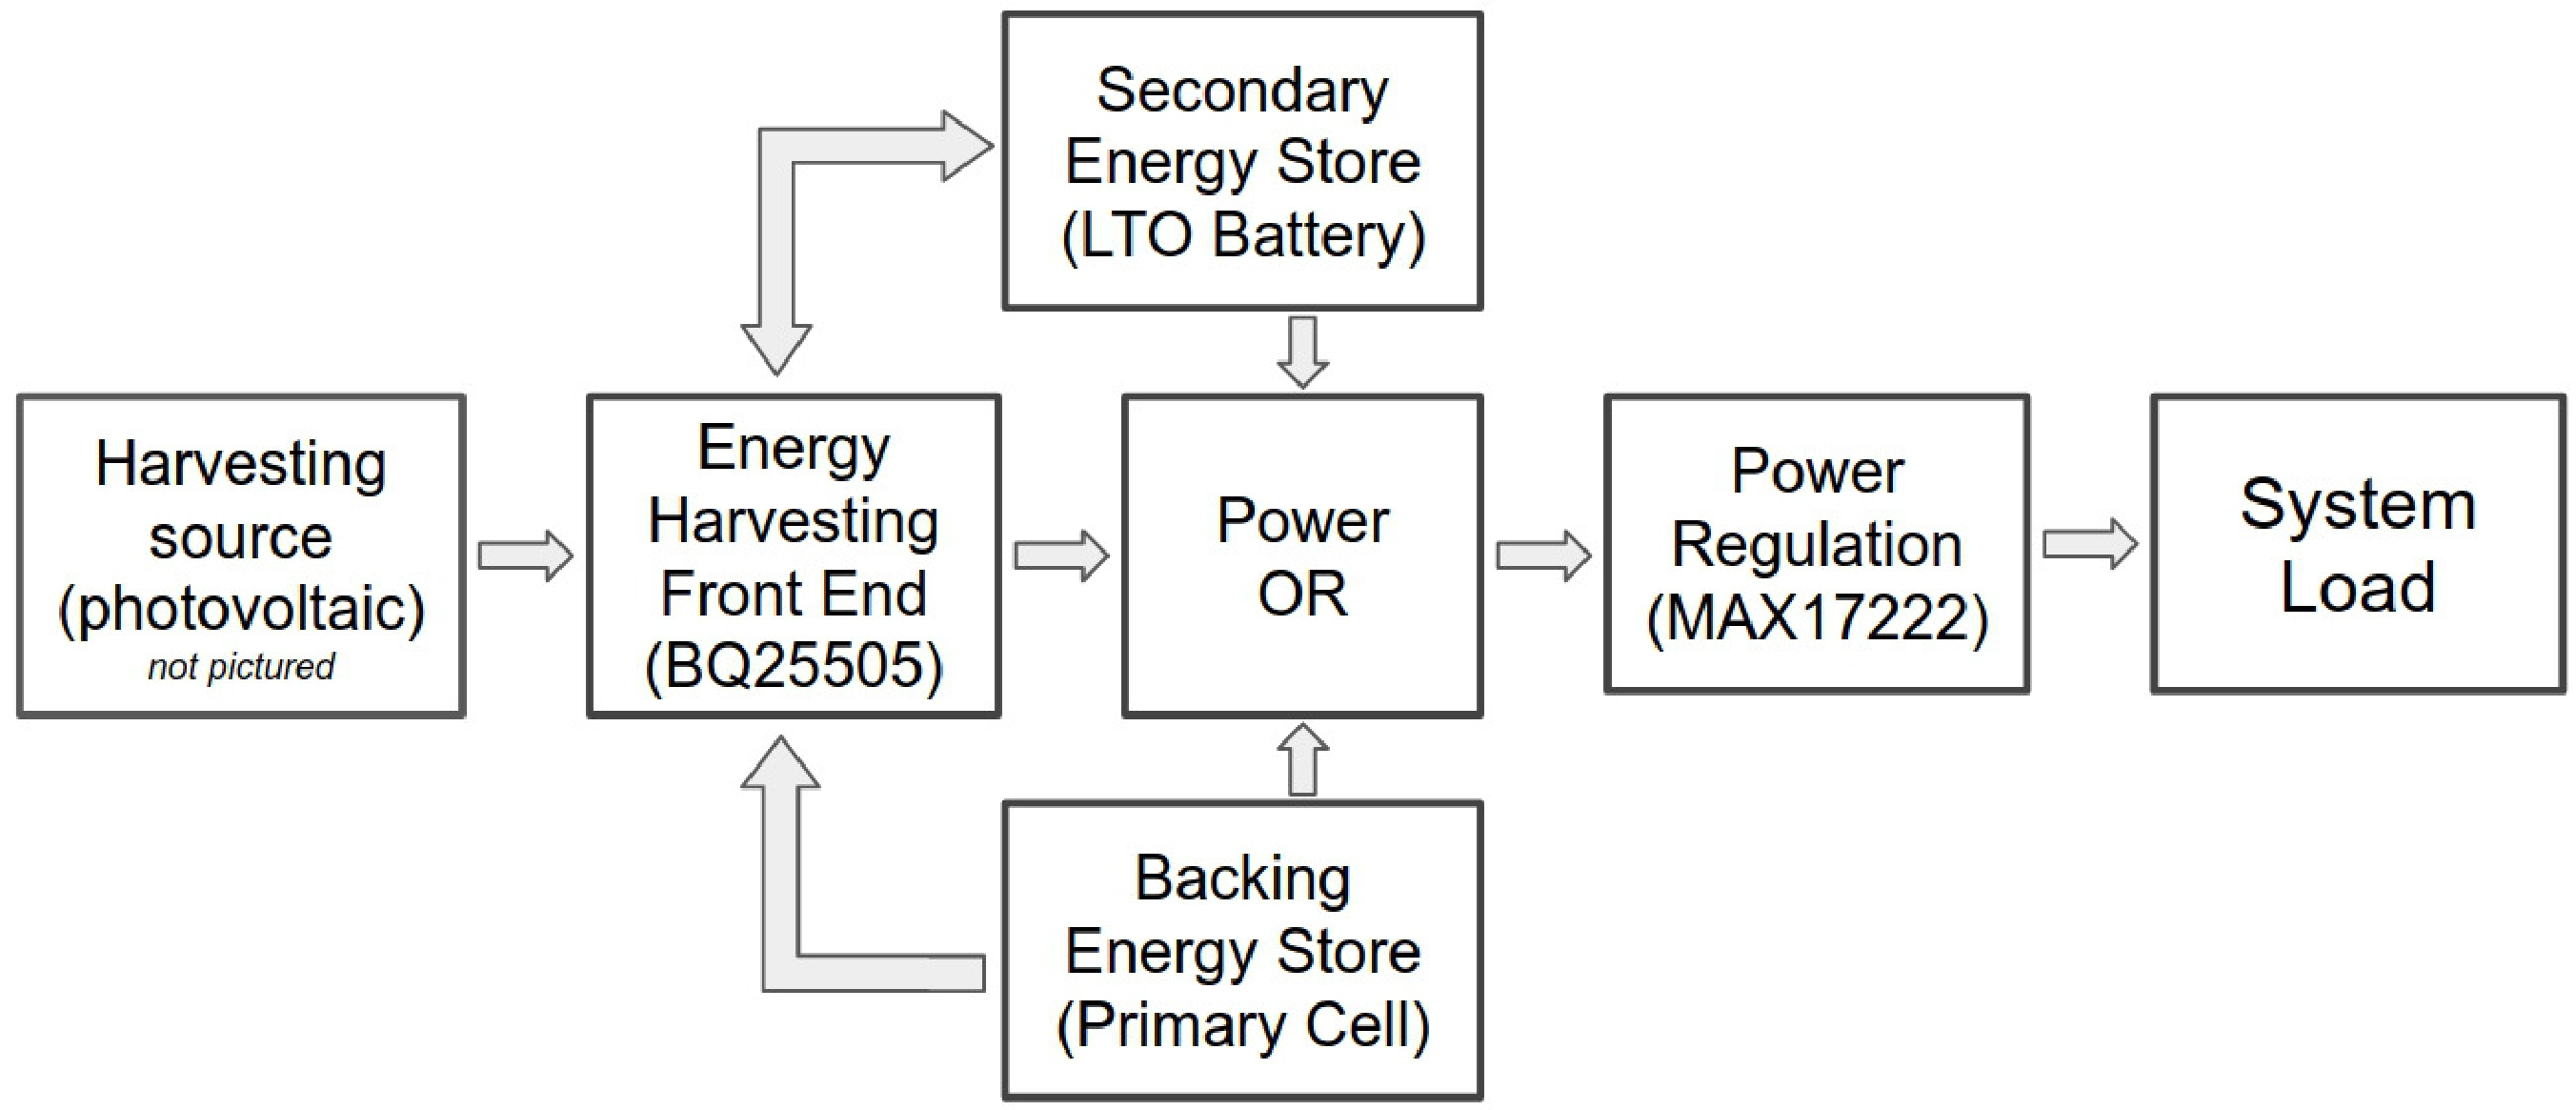
\includegraphics[width=\textwidth]{figs/capacity/arch}
        \caption{Harvesting and storage architecture}
    \end{subfigure}
    \begin{subfigure}{0.29\columnwidth}
        \centering
        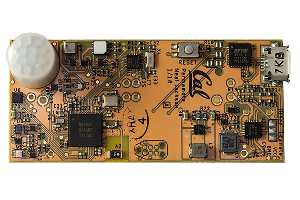
\includegraphics[width=\textwidth,angle=90]{figs/capacity/permamote}
        \caption{Hardware}
    \end{subfigure}
    \caption{\normalfont The \name power supply architecture is informed by the
    findings in \cref{sec:store,sec:primary}. An
    LTO battery is recharged by a solar panel. When the battery is depleted,
    a primary-cell powers the system, providing reliability and avoiding
    intermittency.
    }
    %We believe this platform will run for 6-36 years for common
    %sensing tasks and indoor lighting conditions before the death of
    %the primary-cell. Even after the primary-cell expires,
    %the sensor node could continue to run intermittently on harvested energy.
\end{definefigure}

The advent of LED lighting has significantly reduced electricity consumption in residential and commercial sectors. However, residential and commercial lighting still consumes 5\% of the \textit{total} U.S. electrical consumption~\cite{aeo2022}.
Beyond the utilization of LED lighting, the technique of daylighting, or lighting buildings with natural light, can further reduce the amount of electricity consumed by buildings. 
Since the intensity of daylight can be unpredictable as it depends on weather, it can be difficult to achieve consistent lighting with natural light alone.
Artificial lighting can be used to augment insufficient natural light, but it requires measurement fine-grained feedback and control to accurately maintain a set point in a space.
In particular, workplane illuminance for commercial buildings is important for occupant comfort and productivity, but is difficult to maintain. 
Traditional lighting control systems do not perform fine-grained measurement or control, as the cost of instrumentation is often too exorbitant.
This often results in inequitable and sometimes uncomfortable lighting for occupants.
Wireless sensing could provide a solution for providing measurement for daylighting applications, assuming the sensor is cost-effective, does not require frequent maintenance, and provides high availability and consistent measurements for the lighting system feedback loop.
For this specific example, our application goals are to provide at least a ten year lifetime, provide high availability, and limit cost of individual sensors. 

\placefigure{fig:permamote}

\subsection{Design and Implementation}
We design and implement a prototype sensor named \name to perform workplane illuminance sensing based on the application requirements described previously and the design principals discussed in \cref{chap:capacity,chap:battery}.
%The \name sensing platform
%utilizes the components from the representative hardware listed in \cref{tab:capacity:components} 
%used in our simulation. 
\name integrates a processor, BLE/802.15.4 radio, and various environmental, lighting,
and occupancy sensors. 
The components used in \name are the same ones that we used to develop our representative hardware and workloads for our simulation. 
These components are listed in \cref{tab:capacity:components}. 
A picture
and system diagram of \name is shown in \cref{fig:permamote}. All hardware
and software for the platform is open source\footnote{\url{https://github.com/lab11/permamote/tree/master/hardware/permamote}}.

\subsubsection{Energy Harvesting and Storage.}
Some of the primary goals of \name are to provide periodic workplane illuminance measurements with high availability for a long lifetime of greater than ten years. 
\name is powered by an energy harvesting front end that realizes the benefits
of using batteries. It uses the TI BQ25505 energy harvesting IC, which
harvests energy while monitoring both
rechargeable and backup energy stores,
switching between them at user-configurable voltages~\cite{bq25505}. A
20\,mAh (48\,mWh) LTO battery is charged by an 10.9\ssi{\centi\meter\squared} amorphous
silicon photovoltaic panel~\cite{LTODatasheet, LTODatasheet2}. 
This panel was chosen arbitrarily, however in indoor conditions it can provide between an average of 7--70\ssi{\micro\watt} assuming the bounds of indoor irradiance (10--100\ssi[per-mode=symbol]{\micro\watt\per\centi\meter\squared}). 
We derate the apparent
capacity of this battery to 
elongate the cycle lifetime as described in \cref{sec:battery}, but still have 24\,mWh of
energy storage, more than the capacity required to achieve the reliability and energy utilization
improvements of the intended workload that was simulated in \cref{sec:store}. 
For the backup energy
store, \name uses lithium primary-cells which can be configured to either one or two CR2032 coin
cells or a CR123A cell.
%Primary-cells provide 3-13x more density and 2-12x less
%leakage than a secondary-cell.
%making them more desirable than a single,
%large, pre-charged secondary-cell as the backup store~\cite{LTODatasheet,primary2032, primarycr123a}.
The output of the active battery
is boosted by a MAX17222 regulator, which features high conversion efficiency
(>90\%) at low output currents and operates down to 400\,mV~\cite{max17222}.
%We have the ability to monitor harvesting and system currents using
%the iCount method by sensing the voltage of
%the inductor used by the BQ25505 and MAX17222~\cite{duttaEnergy08}. The processor
%is also capable of gating all sensors from the main power supply to save
%power.\\

\subsubsection{Processor, Radio and Sensor Selection.}
In designing \name, we strive to select modern and low power components.
%We feel that it may
To benefit other
platform builders, we document our component selections
along with their key performance metrics. A summary of these
components can be found in \cref{tab:components}.

We note our choice of the Nordic NRF52840 MCU over the more commonly used MSP430FR series
because of its higher active power efficiency while offering comparable sleep currents.
Specifically, it only draws 56\,\uA/MHz compared to over 100\,uA/MHz
for the MSP430, which is a common choice for batteryless systems. 
Unlike batteryless systems,
\name is designed with sufficient rechargeable capacity and backup energy and is intended to never power off and lose volatile state. 
This reduces the reliance on state retention techniques and eliminates the need for the non-volatile FRAM present on the MSP430FR series chips. 
While
slightly more efficient
processors and radios exist than those found in the NRF52840,
we value the simplicity of an SoC-based design. 

\subsubsection{Energy Benchmarks}
The data presented in \cref{tab:components} are benchmarks taken
on the \name platform. We find that a BLE advertisement at 0\,dbm consumes
86\,\uJ and that sampling both light and color sensors and transmitting
them in a BLE advertisement consumes 586\,\uJ. Additionally, the entire system, including
the energy harvesting front end, consumes only 5.0\,\uW in deep sleep with RAM
retained and all sensors powered off. We use the energy numbers from \name as a basis
for our workloads to fairly compare against prior energy storage architectures.
%\subsection{Numerical Model}
%\label{impl:model}
%
%We develop a numerical model that simulates the behavior of energy harvesting
%systems in indoor environments. For this work, we've primarily focused on solar
%energy input, and have tailored the model to use solar energy traces. As
%mentioned, we use the Columbia EnHANTs irradiance traces
%\cite{margolies2015energy}. We process the traces, filling the few periods of
%missing data by copying from a week prior.
%
%The model operates at second granularity, and at each
%step, the amount of incoming energy is calculated based on the input irradiance
%and solar panel configuration. If the device has enough energy to turn on
%and perform the task from the specified workload it does so. If there is
%energy to spare after the task, the device will enter a low power sleep state.
%The model tallies the amount of successful and unsuccessful events that it
%was expected to complete, as well as the percentage of energy used out
%the energy that was available from the harvesting source. To estimate
%lifetime, the model attempts tasks for the totality of solar irradiance
%data present, then extrapolates primary-cell discharge to find its lifetime
%at empty. The one second granularity imposes some limitations, however
%we find that sensor node workloads are rarely more intensive.
%
%If the secondary store is not at capacity
%this incoming energy is stored
%
%If the device is online, it attempts to turn on
%if it has enough energy to do so, otherwise it remains offline and continues to
%fail performing its workload.  If the device is on, it perform tasks from its
%workload. It prioritizes using the energy from its rechargeable store, and if
%depleted, will either go offline or use energy from its primary-cell, if
%available. If it has energy to spare, it enters a low power sleep state. The
%model tallies the amount of successful and unsuccessful events that it was
%expected to complete, as well as the percentage of energy it used out of how
%much was available from the irradiance source. It also performs a linear fit on
%the primary state of charge to estimate lifetime, if applicable to the
%simulated device's configuration.
%
%This
%granularity also limits that of workloads to a second, but we argue
%that realistic sensor workloads are rarely more intensive \hl{cite}.

\section{Model Evaluation}
\label{sec:eval}
To evaluate the model, we perform a three-month-long deployment in a partially sunlit room
using i) a primary-cell only system, ii) an intermittent, capacitor-only system, and iii) \name, our
system that features both a secondary and primary-cell. We model these
systems over the same period and compare the availability of \name to the
intermittent system.

\subsection{Model Analysis}
\label{sec:eval:model}
We analyze the deployment of these systems
%in a partially sunlit room for three months
and compare their behavior to our
model's predictions: i) ten CR2032 primary-cell only devices, ii) an
intermittent system configured with just 500\textmu F of capacitance (about
0.36\,\textmu Wh at 2.2\,V), and iii) \name, configured with a 20\,mAh
(48\,mWh) secondary-cell, half of which is usable, and a CR2032 backup.  The
primary-cell only device performs environmental sensing over BLE every second.
The intermittent system  sends a beacon as soon as its capacitor bank is full.
When its energy is depleted, it powers off and charges
again. \name is running the ``sense and send'' workload that we described in
\cref{sec:overview}, and sends illuminance measurements every second. This
workload stresses the model and requires more charge and discharge cycles.  We
use \name illuminance readings to estimate irradiance using the same scaling factors used by
Yerva et al.~\cite{yervaGrafting12}, and use these traces as
model input.\\

\vspace{-6pt}
\noindent
\textbf{Primary-Cell Only.}
We model the workload of the primary-cell system and produce estimates for
lifetime.  Our model predicts the platform lifetime
to be 58 days.  We find that the average lifetime of the 10 devices is 61 days.
%,
%from initial deployment to energy depletion, is 61 days.
\\

\vspace{-6pt}
\noindent
\textbf{Intermittent.}
We model the number of packets sent each hour by the
intermittent system over a three week period, and compare against the results of an actual device in
\cref{fig:eval:pkt}.
The average daily error of the model versus our results is 15\%, with a standard deviation of
17\%. This error can attributed to two primary sources. Illuminance is measured
close to, but not exactly at the solar panel of the test device. Occasional
direct sunbeams, like that experienced on day 16, can illuminate the solar
panel but not the sensor, or vice versa. This
results in a substantial over or underestimate of available light. In addition
to inaccurate light measurements, we introduce error through our estimation of
irradiance. We measure illuminance
instead of irradiance, and must resort to a piecewise linear estimation, when
in reality the relationship is not well defined and non-linear when considering
different light sources. In the case of our estimation, results
indicate that the model consistently underestimates high irradiance measurements.\\
\placefigure{tab:components}
\placefigure[t]{fig:evalcmp}

\vspace{-6pt}
\noindent
\textbf{Secondary and Primary-Cell.}
We compare our model's predicted state of charge to a deployed \name over a seven
day period in \cref{fig:eval:soc}. We estimate state of charge from the reported secondary-cell
voltage,
%,
%and measured voltage
%curves of the installed 20\,mAh battery
and irradiance from
lux measurements. In this figure, the state of
charge cycles between configured battery hysteresis limits, as the workload is
too intense to be sustained by energy harvesting alone.
%and the Permamote must
%use energy from its primary cell.
Flat and upward slopes of the curve represent the
device in hysteresis, using the primary battery to perform its workload. Upper slopes
indicate the secondary cell is charging from harvested energy.
Downward slopes indicate the device is out of hysteresis and is using harvested
energy stored in its secondary battery to perform its workload.
%The device is
%charging and in
%hysteresis during upward
%slopes.
The shaded ``nighttime'' regions are not uniform, as the
deployment environment is occupied by graduate students that occasionally work
late hours or forget to turn off the lights.  The model correctly predicts the
cycling
behavior of the deployed device for two days, but deviates
during the third day. The model predicts that the device would charge above the upper
hysteresis limit and begin supplying energy from the secondary-cell before the
test device actually does.  This inaccuracy, like that of the last of
experiment, is partially due to our inexact estimation of irradiance.  In
addition, real device hysteresis limits are set using resistor networks.  The
resistors used have 1-5\% tolerance, and are susceptible to temperature
changes, which introduces dynamic errors that is not accounted for in our model.
Even though the predicted state of charge deviates after two days, the length
and frequency of periods in which harvested energy is stored and used %in the secondary-cell
are identical to our experimental measurements.
%While our model correctly predicts cycling timing and frequency, it appears the
%state of charge  does not quite match that of the measurements.  This is
%because the voltage measured is not the open circuit voltage, and is affected
%by voltage droop due to the applied system load as well as inflated charging
%voltage from the energy harvesting front end.  Ignoring these effects, the
%cycling of the model's prediction is closely synchronized with the estimated
%state of charge.
%We compare the model's predicted
%state of charge over time to the outputs of systems we
%have deployed. For energy harvesting systems we collect lux measurements
%throughout the deployment and convert lux to irradiance based on the
%data collected in Yerva et al.~\cite{yervaGrafting12}. \\
%\vspace{-6pt}
%\noindent
%\textbf{Permamote.}\\
\subsection{\name Performance}
\placefigure[t]{fig:eval}
\label{sec:eval:permamote}
%In addition to evaluating our model,
We also compare the performance of the
deployed intermittent system and \name. In \cref{fig:evalcmp}, we show the
number of packets sent per hour for two days. \name sends data every
second, while the intermittent system sends as fast as possible. \name is
able to collect and send its data continuously, while the
intermittent system is limited to sending only during the day. This
demonstrates the increased availability afforded by increasing secondary
capacity and including a backup energy store.

We also use our model to explore the estimated performance of \name
compared to prior systems.
To isolate the analysis to just power supply types and sizing, we assume each
system uses the same low-power hardware and is performing the same workload.
The results of this modeling are shown in \cref{tab:related}. Our model estimates that
\name can expect several decades of 100\% reliable lifetime when configured as
it was deployed for this evaluation, albeit configured with a less intense workload.
%While the workload used with \name is not
%sustainable for the multi-decade lifetimes we are targeting, it still
%exemplifies the increase in reliability afforded by including a primary-cell.


\begin{definefigure}{fig:eval}
  \centering
  \begin{subfigure}{\columnwidth}
    \centering
    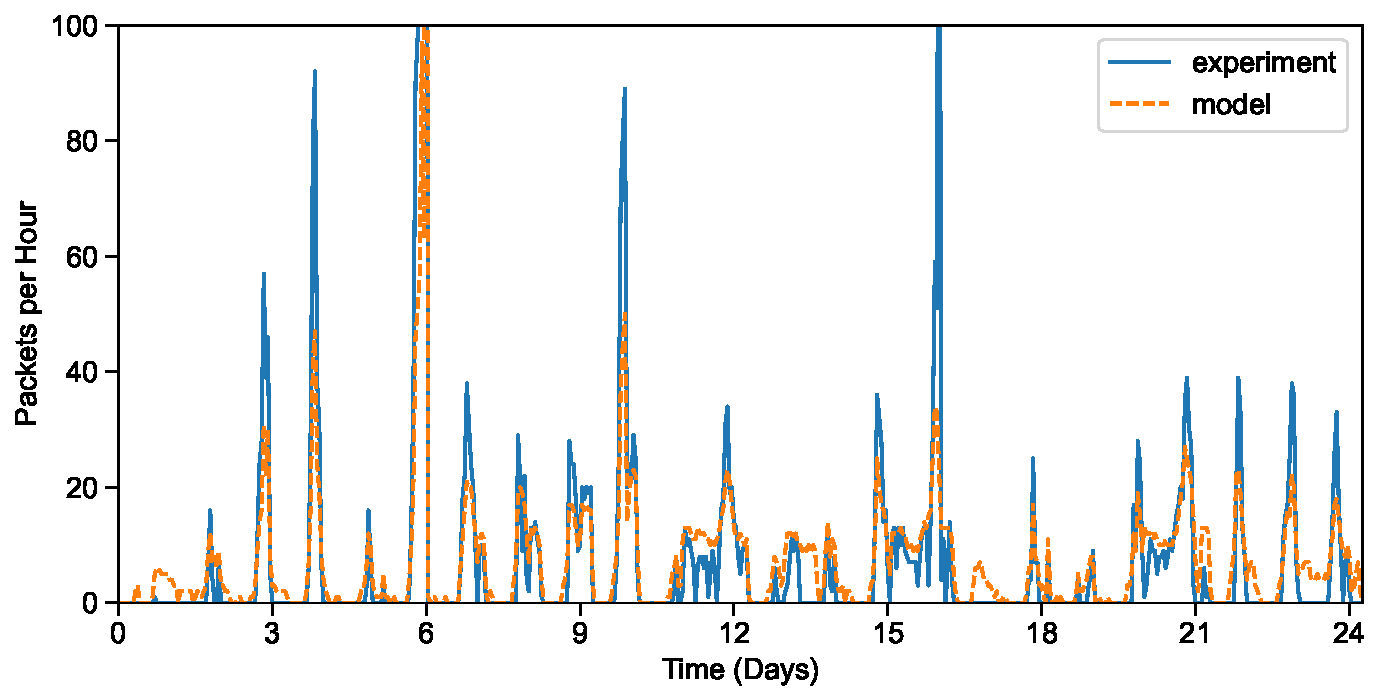
\includegraphics[width=\linewidth]{figs/capacity/experiment_pkt/exp_vs_sim_pkt}
    \caption{Intermittent Node}
    \label{fig:eval:pkt}
  \end{subfigure}\\%\hspace{0.5cm}
  \begin{subfigure}{\columnwidth}
    \centering
    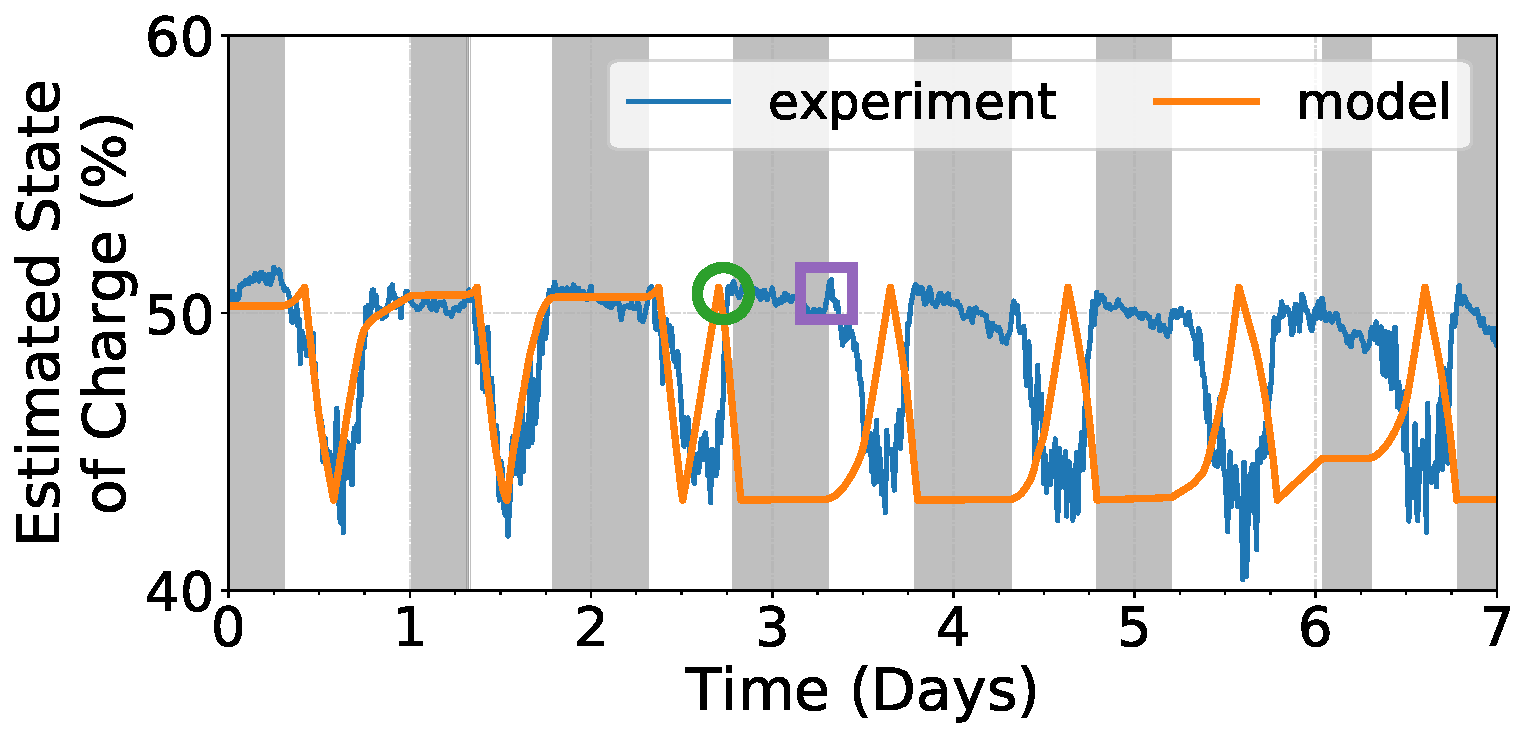
\includegraphics[width=\linewidth]{figs/capacity/experiment_soc/exp_vs_sim_soc}
    \caption{Permamote}
    \label{fig:eval:soc}
  \end{subfigure}
    \caption{Model comparison to deployed hardware.
    \normalfont
    Data from a three month deployment of two systems is used to verify our model.
    (a) We use three weeks of lux measurements %from a month-long deployment
    to estimate irradiance and model the number of packets transmitted by an
    intermittent node. Average daily error is 15\%, with a standard deviation
    of 17\%. (b) We model and measure a \name's state of charge while running a
    ``sense and send'' workload with a 1\,s period for a week, beginning at
    midnight on the first day. Secondary charging hysteresis
    limits of the devices are set at 51\% and 43\%. Shaded regions
    represent periods of low harvestable potential
    (<\,15\,\textmu W/cm\textsuperscript{2}),
    i.e. nighttime. For the first two days, model predictions
    closely track the experimental measurements. Errors
    in hysteresis and irradiance estimation cause the model to reach its upper
    hysteresis sooner than the experiment does, annotated by the
    \textbf{\textcolor{fig-green}{green circle}}. In actuality, the device
    exits charging hysteresis at the peak marked with the
    \textbf{\textcolor{fig-purple}{purple square}}.
    More importantly, the
    frequency and length of periods spent using harvested
    energy collected in the secondary-cell (downward slopes) are identical.
    %For the intermittent node we see our model
    %underestimate the number of transmitted packets by 10-20\% except for the
    %first day which predicts significantly more packets.  We believe this error
    %is primarily due to a piecewise linear estimation of irradiance from our
    %collected illuminance data, when in reality the relationship is complex and
    %non-linear.  For (b) we estimate the state of charge of \name
    %based on the secondary
    %cell voltage. Differences between the estimated state of charge and the
    %modeled state of charge are primarily due to inflated voltage during
    %charging and voltage droop and bounce back when \name
    %draws current from the secondary-cell.
    %Even though estimated state of
    %charge is not accurate due to this voltage swing, it is clear that the
    %timing of charge and discharge aligns between the model and the
    %experimental data.
    }
\end{definefigure}

\begin{definefigure}{fig:evalcmp}
    \centering
    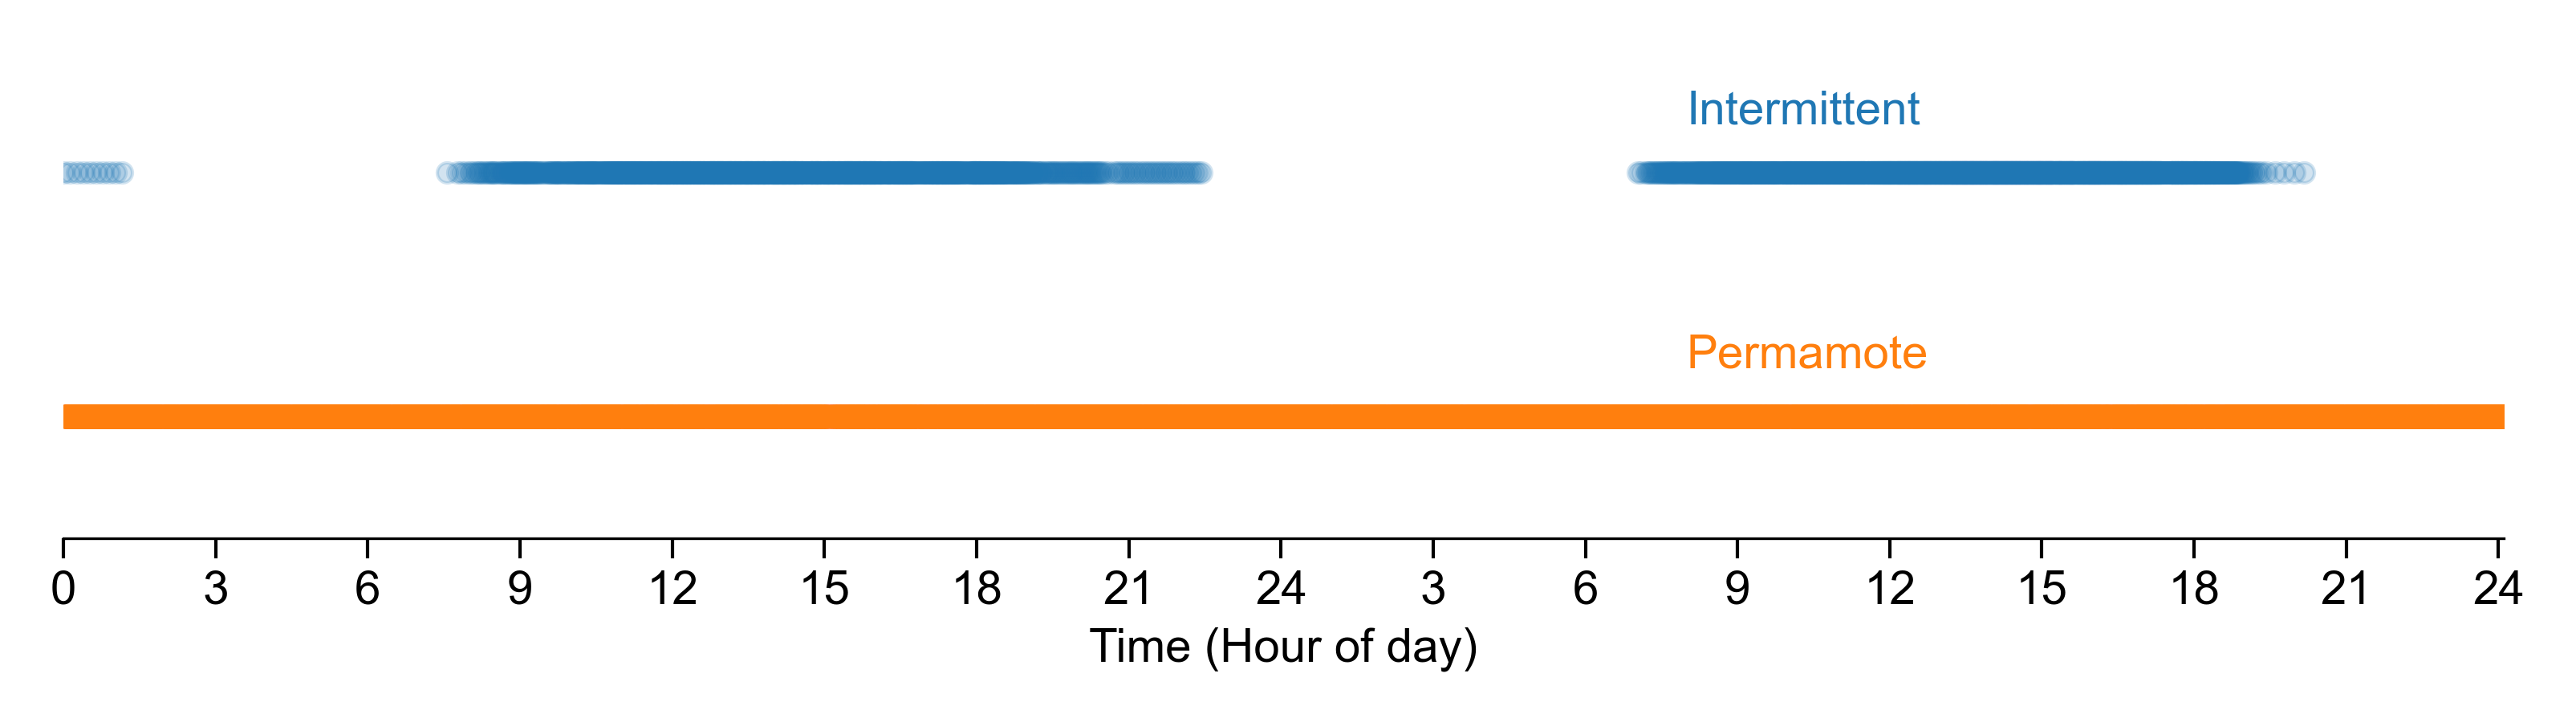
\includegraphics[width=\linewidth]{figs/capacity/experiment_sys_compare/exp_packets_recv}
    \caption{
      \normalfont
        Packets received over two days.
      This figure compares the reliability of an
      intermittent design and \name. \name sends a packet every second and does
      so without fail, while the intermittent system is only able to send when
      light is available.
      %This results in periods at night where the
      %intermittent device does not harvest enough energy to sustain operation.
      }
\end{definefigure}
\placefigure{tab:related}

% what does power subsystem need to provide? 
% upsizing battery? what are interfaces
% as you increase size of charge buffer, size of amount of buffering you have for small variations goes away
% big cap squelch high frequency, keep increasing further and further, squelch over day, week, year
%contininuity of buffer, hard to reason over intermittency, easy to reason about how to buffer over it
%0.1uF noise, 10 uF surge, larger 100uF stabilize power supply, even larger mF operate store charge for a workload, only good for one activation
%continium on buffer capacity

\section{Evaluating an Existing System through Simulation}

\section{Capacity-focused Redesign of an Existing System}


\section{Summary}